\section{Round dances and carry-over effects}\label{sec:round-dances}

\topic{Lucas's round dances}

In the second volume of his \emph{R\'ecr\'eations math\'ematiques} (1883), Lucas~\cite{luc1883} posed the following problem under the title ``Les rondes enfantines''.

\begin{problem}[Lucas, 1883]\label{prob:lucas}
Children dance in a ring, holding hands. How should the children be placed in successive rounds so that each child is, in turn, a neighbour of every other child, on the right or on the left, but only once?
\end{problem}

The solutions Lucas prints are due to Walecki, who taught at the Lyc\'ee Condorcet. Lucas observed a necessary condition. In every round a child has two neighbours, and no pair may meet twice, so each child meets the others two at a time; hence the number of \emph{other} children is even. So there are $2n+1$ children, and there must be exactly $n$ rounds. In graph language, the problem asks for a decomposition of $K_{2n+1}$ into $n$ Hamilton cycles.

For eleven children Lucas gives five rounds; child \texttt{A} stands in the centre of the figure below.
\begin{center}
\begin{tabular}{rl}
I & \texttt{A B C D E F G H I J K A}\\
II & \texttt{A C E B G D I F K H J A}\\
III & \texttt{A E G C I B K D J F H A}\\
IV & \texttt{A G I E K C J B H D F A}\\
V & \texttt{A I K G J E H C F B D A}
\end{tabular}
\end{center}
All $55=\binom{11}{2}$ pairs of children are neighbours exactly once. Walecki's construction is a ``needle'' (Figure~\ref{fig:walecki}): put one child at the centre, labelled $\infty$, and ten on a circle; the zigzag together with the two dashed edges is one round, and rotating the needle by one step gives the next round.

\begin{figure}[ht]
\centering
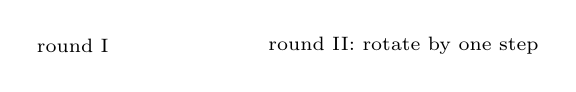
\begin{tikzpicture}[every node/.style={font=\scriptsize}]
    \waleckiPanel{0}{0}{col1}
    \waleckiPanel{4.2}{1}{col2}
    \node at (0,-2.0) {round I};
    \node at (4.2,-2.0) {round II: rotate by one step};
  \end{tikzpicture}

\caption{Walecki's needle for eleven children. Rotating it by one step gives the next round.}
\label{fig:walecki}
\end{figure}

\topic{Where the group is hiding}

Label the $2n$ outer children by $\Z_{2n}$. Walecki's zigzag is
\[
a=(0,\,1,\,2n-1,\,2,\,2n-2,\,3,\,\dots,\,n),
\]
which for $2n=10$ is $0,1,9,2,8,3,7,4,6,5$. Its successive differences are $1,-2,3,-4,\dots$, that is,
\[
b=(1,\,2n-2,\,3,\,2n-4,\,\dots),
\]
which for $2n=10$ is $1,8,3,6,5,4,7,2,9$: every non-zero element of $\Z_{2n}$ exactly once.

\begin{fact}[Ollis~\cite{oll25}, Example~4]\label{fact:walecki}
The $n$ rotations $a+i$, $0\leq i<n$, decompose $K_{2n}$ into Hamilton paths, and joining the ends of each to $\infty$ gives Lucas's $n$ rounds. All $2n$ rotations, read as directed paths, decompose the complete digraph on $\Z_{2n}$ into $2n$ directed Hamilton paths.
\end{fact}

We have checked this for $2n=10$. The ordering $(0,b)$ will reappear in Section~\ref{sec:sequenceable} as the Lucas--Walecki sequencing of $\Z_{2n}$.

\topic{Williams's designs}

Williams~\cite{wil49} considered in 1949 an experiment in which $n$ treatments, for instance diets, are given in succession to the same units, for instance cows: each unit receives all $n$ treatments, one per period. With the units as rows and the periods as columns this is a Latin square. The difficulty is that the response in a period depends not only on the treatment given then (the \term{direct effect}) but also on the treatment of the previous period (the \term{residual} or \term{carry-over effect}),
\[
y=\mu+\text{unit}+\text{period}+\tau_{\text{now}}+\rho_{\text{before}}+\varepsilon .
\]
To estimate all the $\rho$'s equally well, every treatment should be preceded by every other treatment equally often. Williams's example concerned diets and the milk yield of cows~\cite[\S3.6]{oll25}; Figure~\ref{fig:cows} shows such a square for four treatments.

\begin{figure}[ht]
\centering
\begin{tikzpicture}[every node/.style={font=\small}]
    \foreach \row [count=\i] in {{0,3,1,2},{1,0,2,3},{3,2,0,1},{2,1,3,0}}
      \foreach \c [count=\j] in \row
        \node[lscell, minimum size=6.5mm] at (0.65*\j, -0.65*\i) {$\c$};
  \end{tikzpicture}

\caption{Four cows, four periods, four diets: each diet follows each other diet exactly once.}
\label{fig:cows}
\end{figure}

\begin{theorem}[Williams~\cite{wil49}]\label{thm:williams}
A design balanced for the effect of the preceding treatment exists with $n$ replications, that is with one $n\times n$ square, when $n$ is even, and with $2n$ replications, that is with two squares, when $n$ is odd.
\end{theorem}

For $n=3$ one square cannot work: none of the $3\times3$ Latin squares has all six ordered pairs adjacent in its rows. Williams's two squares for $n=3$ are shown in Figure~\ref{fig:williams-three}. This raises the question for which odd $n$ a single square suffices.

\begin{figure}[ht]
\centering
\begin{tikzpicture}[every node/.style={font=\small}]
    \foreach \row [count=\i] in {{0,1,2},{1,2,0},{2,0,1}}
      \foreach \c [count=\j] in \row
        \node[lscell, minimum size=6.5mm] at (0.65*\j, -0.65*\i) {$\c$};
  \end{tikzpicture}\qquad
\begin{tikzpicture}[every node/.style={font=\small}]
    \foreach \row [count=\i] in {{2,1,0},{0,2,1},{1,0,2}}
      \foreach \c [count=\j] in \row
        \node[lscell, minimum size=6.5mm] at (0.65*\j, -0.65*\i) {$\c$};
  \end{tikzpicture}

\caption{For $n=3$ the second square reverses the rows of the first. Together, each ordered pair is adjacent twice.}
\label{fig:williams-three}
\end{figure}

\topic{Row-complete Latin squares}

\begin{definition}[Ollis~\cite{oll25}, \S1]\label{def:row-complete}
A Latin square is \term{row-complete} if every ordered pair $(x,y)$ with $x\neq y$ occurs exactly once in horizontally adjacent cells. It is \term{complete} if it is also column-complete.
\end{definition}

For $n$ symbols, the following are three faces of the same object: a Williams design for $n$ treatments using one square; a row-complete Latin square of order $n$; and a decomposition of the complete digraph on $n$ vertices into $n$ arc-disjoint directed Hamilton paths, obtained by reading the rows as paths.

\begin{fact}[Ollis~\cite{oll25}, \S1]\label{fact:row-complete}
A row-complete Latin square of order $n$ decomposes the complete digraph on $n$ vertices into $n$ arc-disjoint Hamilton paths: each row visits every vertex once, and each ordered pair is used once.
\end{fact}

\begin{figure}[ht]
\centering
\begin{tikzpicture}[>=Latex, every node/.style={font=\footnotesize}]
    \hamPanel{0}{col1}{0}{3}{1}{2}
    \hamPanel{3}{col2}{1}{0}{2}{3}
    \hamPanel{6}{col3}{3}{2}{0}{1}
    \hamPanel{9}{col4}{2}{1}{3}{0}
  \end{tikzpicture}

\caption{The rows of the square of Figure~\ref{fig:cows} as paths. The $12$ arcs are distinct, so they are all the arcs of the complete digraph on $4$ vertices.}
\label{fig:ham-paths}
\end{figure}
